\documentclass[../FinalThesis.tex]{subfiles}
\begin{document}
\chapter{General Discussion}
\label{GeneralDiscussion}
\thispagestyle{empty}
\vspace{-1cm}
\noindent\hfil\rule{0.75\textwidth}{.4pt}\hfil

\newpage

\section{A Fresh Take on Connectivity}

In this thesis, I explored several critical factors linked to various aspects of
dispersal and landscape connectivity. In \Cref{ChapterSimulation}, I introduced
a novel approach to assess functional landscape connectivity via simulated
dispersal from iSSFs and demonstrated its application using GPS data from
dispersing AWDs. In \Cref{ChapterFlood}, I used the newly developed approach to
reveal potential differences in connectivity for dispersing AWDs under varying
environmental conditions in the context of ongoing climate change. In
\Cref{ChapterSeasonality}, I examined the importance of seasonal dynamism and
investigated how the inclusion of seasonality affects dispersal simulations and
inferred patterns of connectivity. Lastly, in \Cref{ChapterIrregularity}, I
revisited the iSSF framework employed throughout Chapters 2 to 4, and proposed
various methods to generalize the framework for application in scenarios where
GPS data exhibit temporal irregularities.

Probably the most pressing question with regard to the investigated factors is
whether they actually matter for our understanding of connectivity, and whether
their consideration alters our insights into conservation. If we qualitatively
compare the connectivity maps generated from my master's thesis
\citep{Hofmann.2021} and the various chapters of this doctoral thesis
(\Cref{MapComparisonChapters}), the sobering answer would probably be a simple
no. While the maps may not be entirely identical, they appear qualitatively
similar. This is insofar surprising, as the maps were generated using rather
different approaches and simulation parameters. One may conclude that these
differences do not warrant the additional efforts of parameterizing a
mechanistic IBMM and addressing several typically overlooked limitations, thus
resolving to traditional, presumably simpler, methods to model connectivity.
However, such a view would overlook various improvements that are achieved
``under the hood'' and I will argue that it is precisely these improvements that
increase our ability to simulate dispersal and quantify connectivity to a new
level.

\begin{figure}[htpb]
  \begin{center}
  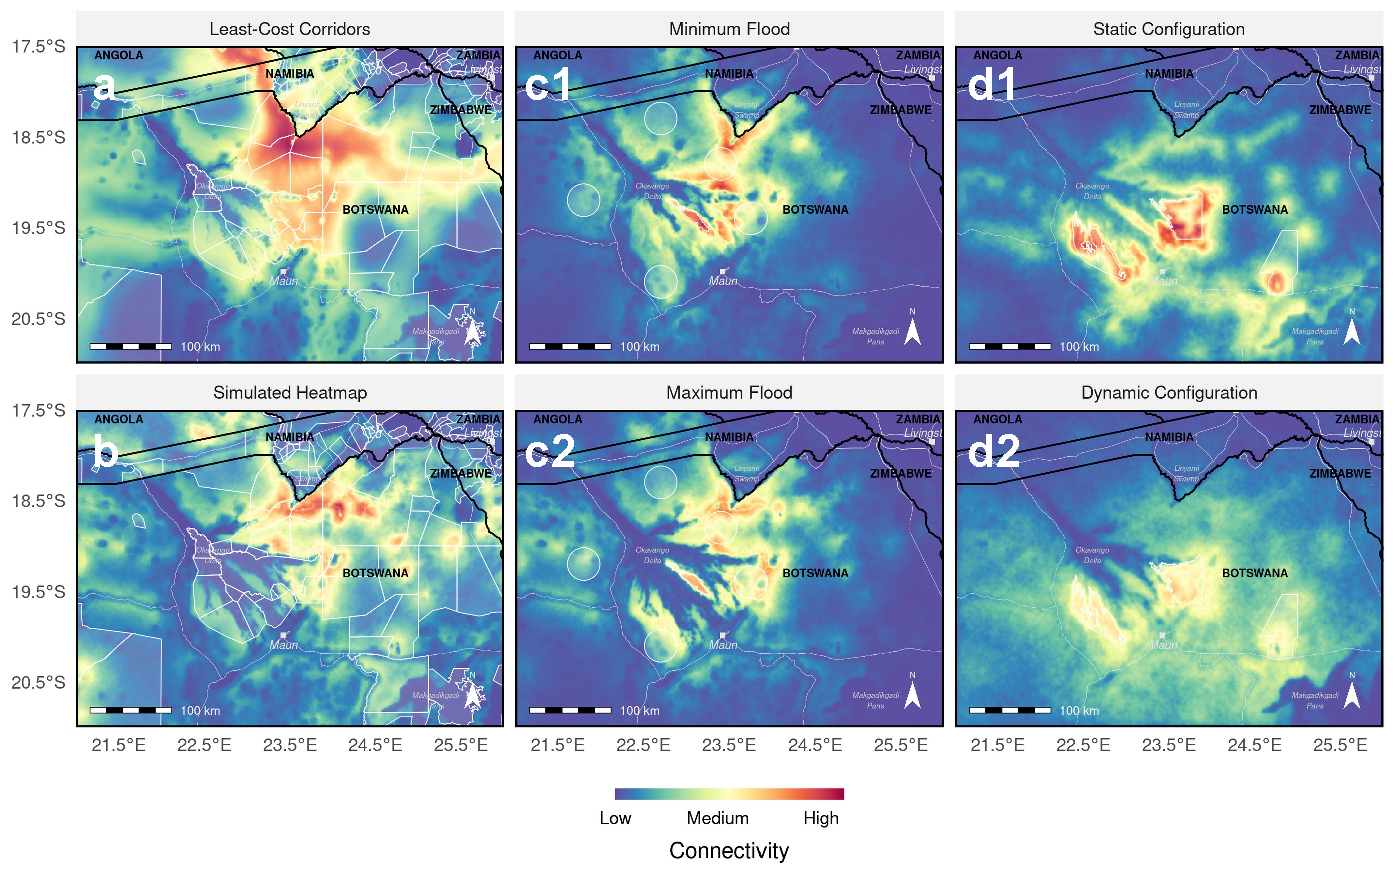
\includegraphics[width = \textwidth]{Figures/MapComparison.pdf}
  \caption{Comparison of the connectivity maps resulting from my master's thesis
  and throughout the chapters of this PhD thesis. Since methodology, data,
  covariates, and source areas (semi-transparent white polygons) differed from
  chapter to chapter, this should be considered a qualitative comparison. (a)
  Least-cost corridors computed between national parks and protected areas,
  computed as part of my master's thesis \citep{Hofmann.2023}. (b) Heatmap
  emerging after simulating dispersal trajectories using the three-step approach
  introduced in \Cref{ChapterSimulation}. (c1, c2) Heatmaps produced from
  simulated dispersal trajectories under the minimum flood extent and maximum
  flood extent in \Cref{ChapterFlood}. (d1, d2) Heatmaps produced from simulated
  dispersal trajectories in a fully static and dynamic configuration in
  \Cref{ChapterSeasonality}.}
  \label{MapComparisonChapters}
  \end{center}
\end{figure}

A major benefit of using iSSF-based IBMMs over traditional connectivity modeling
methods is that they bypass the necessity for a permeability surface
\citep{Diniz.2019, UnnithanKumar.2022a}. Permeability surfaces are often based
on arbitrary conversions from habitat suitability to habitat permeability
\citep{Zeller.2018}, yielding unconditional predictions of a species' ability to
move and disperse \citep{Signer.2017}. Essentially, this implies that the
permeability of an area (i.e. of a single grid-cell) is solely determined by the
area's characteristics, without consideration of possible alternatives. This is
in direct contradiction to the conditional logistic regression models that are
normally utilized to parameterize such permeability surfaces
\citep{Zeller.2012}; these are inherently based on the principle of conditional
probabilities \citep{Avgar.2017}. In reality, it can also be assumed that an
animal's willingness to traverse a specific area is contingent on what is
available elsewhere. For instance, an animal encountering a densely populated
human area may find the alternative of moving into a forest more appealing than
if it were currently situated in open Savannah habitat. A conditional prediction
therefore seems more appropriate, and is precisely what is achieved through
iSSF-based IBMMs \citep{Signer.2017}.

Utilizing a mechanistic movement model to simulate dispersal also opens up new
avenues for incorporating factors that play an important role in reality. In
\Cref{ChapterSimulation}, for instance, I accounted for the fact that movement
behavior depended on habitat characteristics by including interactions between
step-descriptors and habitat covariates. In \Cref{ChapterFlood}, I further
modeled that dispersal movements depend on temperature and light availability.
Incorporating such intricacies using permeability-based connectivity models is
simply not feasible, as they lack a mechanistic understanding of movement
\citep{Zeller.2012}. Instead, permeability-based models adopt a series of
simplistic grid-based movement rules that govern how individuals move from one
grid-cell into a neighboring one. This also implies that the resolution of
spatial covariates determines the presumed perception radius the focal species,
as well as the temporal scale at which it moves across the landscape
\citep{Diniz.2019}. iSSF-based IBMMs overcome this limitation and instead permit
to create models that allow animals to traverse multiple grid-cells in a single
go, thus extending their landscape perception to a more meaningful distance. By
simulating dispersal trajectories in space and time, the output of an iSSF-based
IBMM is not limited to a single map, but allows preparing a suite of
complementary connectivity metrics that provide a more nuanced and comprehensive
view on a system's landscape connectivity \citep{Diniz.2019}. In
\Cref{ChapterSimulation}, I suggested preparing the metrics inter-patch
connectivity, betweenness, and traversal frequency (heatmap), as each of those
focuses on a different aspect of connectivity.

The realization that connectivity need not be confined to a single metric
alludes to another problem in current connectivity studies, namely that they all
exhibit a slightly different understanding of what connectivity actually
entails. While many studies readily cite \citet{Taylor.1993}'s definition of
connectivity, they typically employ very different methods and metrics to
quantify it. Some studies gauge connectivity through the strength of association
between different habitats as measured based on observed or simulated movements
(e.g., \citealp{Revilla.2008, Kanagaraj.2013, Dilts.2016}), while others assess
it by focusing on the matrix between such habitats \citep{Etherington.2016,
Diniz.2019}. The latter group can again be separated into studies that estimate
permeability within their study area (e.g. \citealp{Martin.2018}), studies that
estimate the intensity of use of different areas (e.g. \citealp{Zeller.2020}),
and studies that attempt to identify distinct movement corridors (e.g.,
\citealp{Elliot.2014, Benz.2016, Brennan.2020}). Undoubtedly, each of these
approaches is valid for capturing some aspect of connectivity, albeit they all
focus on a slightly different one. Therefore, I propose to reconsider the term
``connectivity'' by viewing it as an overarching concept that can be further
subdivided into the dimensions of connectedness, conductance and betweenness. I
would define these terms as follows:

\begin{itemize}

  \item \textbf{Connectedness:} Connectedness refers to the degree to which
  different patches or habitats within a landscape are functionally connected.
  It measures the ease and frequency with which organisms can move between
  different areas of the landscape. I have previously investigated this aspect
  of connectivity via \textit{Inter-Patch Connectivity Maps}.

  \item \textbf{Conductance:} Conductance describes the degree to which the
  landscape allows movement or flow of organisms across it. It considers factors
  such as habitat structure, land use, and barriers that affect the ability of
  organisms to move through the landscape. I have previously investigated this
  aspect of connectivity via \textit{Heatmaps}.

  \item \textbf{Betweenness:} Betweenness quantifies the importance of different
  elements of the matrix in facilitating connectivity between other patches or
  habitats within the landscape. It identifies key corridors or bottlenecks that
  serve as critical links for maintaining overall connectivity in the landscape.
  I have previously investigated this aspect of connectivity via
  \textit{Betweenness Maps}.

\end{itemize}

Adopting this terminology and acknowledging that connectivity can be
multidimensional would greatly facilitate navigating the confusing diversity of
connectivity literature and connectivity  modeling approaches, and help to
clarify what dimension of connectivity they measure. A major benefit of using
iSSF-based IBMMs over permeability-based approaches is that they permit
statements about all three dimensions, thus offering a holistic view on
connectivity patterns.

\section{Conservation Insights}

Even though my chapters were primarily focused on methodological aspects, their
results permit several conclusions on the conservation of AWDs, as well as on
some ecological principles. Probably the most important result is that the AWD
population studied in this thesis appears to benefit from a comparably high
degree of connectivity. This is a testimony to the area's pristine condition and
relatively low human disturbance, which permit dispersing coalitions to roam
relatively unhindered in their pursuit to find potential mates and a new
territory. Moreover, the planned KAZA-TFCA initiative appears to align well with
many of the critical dispersal routes between existing national parks and
wildlife management areas, thereby providing an effective means to safeguard the
species' ability to disperse. I arrived at this conclusion already in my
master's thesis \citep{Hofmann.2021}, but the results of this PhD thesis further
corroborate this notion. Notably, GPS data collected on dispersing coalitions
revealed several successful dispersal events from BPC's study area into
surrounding, less pristine habitats. The study population, which is currently
considered a stronghold population, may thus considerably contribute to the
recolonization of surrounding habitat patches and reinforcement of weakened
subpopulations. Besides this, my dispersal simulations from
\Cref{ChapterSimulation} revealed that the study area in northern Botswana
likely acts as a major dispersal hub where several dispersal routes that run
across the KAZA-TFCA ecosystem are funneled due to natural and human
impediments. The protection of this area therefore plays a crucial role in
conserving AWDs, particularly in light of ongoing climate change. As
demonstrated in \Cref{ChapterFlood}, climate change holds the potential to
disrupt and rearrange preferred movement corridors, thus leading to the
emergence of novel hotspots for human wildlife conflict. Initiatives aimed at
raising awareness and educating affected communities, as well as the
implementation of appropriate prevention and compensation systems, will help
ensure greater acceptance by the local population. Finally, I motivated in
\Cref{ChapterSeasonality} that connectivity should not be viewed as a static
property but rather as a dynamic and multidimensional concept. Although I found
that the incorporation of seasonality only marginally improved the predictive
power of dispersal models, inferred connectivity patterns differed
significantly. In particular, a seasonal take at connectivity appeared to result
in connectivity being more homogeneously distributed than what was suggested by
a static analysis. This was likely due to seasonally available dispersal
habitats. A more holistic perspective must be adopted for the successful
conservation of dispersing species, as conservation measures cannot be limited
to preserving highway-like corridors, but should be broadened to encompass the
diversity of dispersal routes emerging under dynamic environmental conditions.

\section{Methodological Considerations and Limitations}

The additional realism and flexibility gained by moving from permeability-based
connectivity assessments to an iSSF-based IBMM, and the novel insights gained
from studying the impacts of climate change and seasonality come at considerable
costs, both in terms of data and computational requirements. For example,
parameterizing an IBMM via iSSFs necessitates GPS data on the study species
\citep{Fortin.2005, Thurfjell.2014, Avgar.2016}, preferably collected during
dispersal \citep{Elliot.2014}. In many instances, GPS data or data during
dispersal are unavailable (e.g. \citealp{Jackson.2016, Day.2019, Day.2020}). In
this case fitting an iSSF is simply not possible, and the modeler needs to
revert to a traditional connectivity model. Similarly, data on on-the-ground
conditions under climate change or seasonality can be challenging to collect.
Seasonal data can sometimes be obtained via remote sensing, which has become
vastly facilitated thanks to centralized data hubs (e.g., Google Earth Engine).
Nevertheless, the incorporation of seasonality necessitates handling large
data-volumes and dealing with noise due to missing values or cloud cover. A
seasonal take at connectivity also requires splitting the input data by season,
which can substantially reduce the amount of data remaining to inform
habitat-selection and movement behavior in distinct seasons. Similarly,
obtaining information on environmental conditions under climate change remains
difficult \citep{Littlefield.2019}. Spatial data on atmospheric conditions may
be readily available (e.g., \citealp{CopernicusClimateChangeService.2021}), yet
these are rarely translated into on-the-ground information on land-cover and
land-use, thus limiting their usefulness for connectivity studies (but see
\citealp{Sleeter.2018}). In \Cref{ChapterFlood}, I proposed exploiting seasonal
extremes to gauge the likely impacts of climate change on environmental
conditions, yet this remains a poor proxy for long-term shifts in the biosphere.
Either way, the benefits gained by increasing realism need to be carefully
balanced against the potential costs of doing so \citep{Puy.2022}.

In \Cref{ChapterSimulation}, I highlighted that connectivity studies entail
numerous non-trivial modeling decisions \citep{Beier.2008}. These encompass the
selection of suitable species data and covariate layers \citep{Elliot.2014,
Fattebert.2015, Finerty.2023}, as well as the choice of an adequate spatial and
temporal scale \citep{Zeller.2014, Zeller.2017, Ciudad.2021}. For iSSF-based
IBMMs, additional modeling decisions emerge (\Cref{ModelingDecisions}),
including how to deal with individual variability, the number and placement of
starting points, and the behavior of simulated individuals at map boundaries
\citep{Diniz.2019}.

For permeability-based connectivity studies, several useful reference works and
overviews that help with the application of established approaches and the
associated decision-making processes exist \citep{Beier.2008, Beier.2011,
Zeller.2012, Etherington.2016, Zeller.2018, Diniz.2019, Hilty.2020}. It is
imperative that analogous reference material is developed for iSSF-based IBMMs,
both to facilitate the uptake and application of new methods, as well as to
maintain comparability of studies from different species and systems. As already
motivated by \citet{Finerty.2023}, maintaining comparability between
connectivity studies is of central importance to distinguish biological
differences from methodological artifacts. This holds particularly true for
methods that exhibit greater flexibility and thus higher variability in
outputted results. In this context, comprehensive sensitivity analyses will
become of great importance, as they serve to pinpoint simulation parameters that
require particular attention due to their disproportionate impact on the
resultant connectivity patterns \citep{Kanagaraj.2013}. Quantifying the
sensitivity of non-spatial metrics to simulation parameters is straightforward.
However, extending a sensitivity analysis to spatial metrics, such as
betweenness or conductance, seems more involved. In simple cases, connectivity
maps emerging under different scenarios can simply be contrasted using
difference maps (e.g., \citealp{Day.2020}). I have applied the same technique in
\Cref{ChapterFlood} to highlight differences in connectivity between the maximum
and minimum flood scenario. An alternative approach is provided by
\citet{Marrec.2020}, who assess the sensitivity of their connectivity outputs by
comparing connectivity values via violin-plots and map-correlations.
Unfortunately, this approach fails to provide a spatial depiction of
sensitivities. I therefore propose yet another solution, which is to simulate
connectivity under varying parameters and generate the spatial metrics of
interest (e.g., heatmap, betweenness map, etc.). Then, one can apply
grid-cell-wise linear regression to quantify how strongly the value of each
grid-cell responds to changes in simulation parameters. The benefit of this
approach is that it allows visualizing sensitivity spatially, thus highlighting
areas that require particular attention.

\begin{figure}
  \begin{center}
  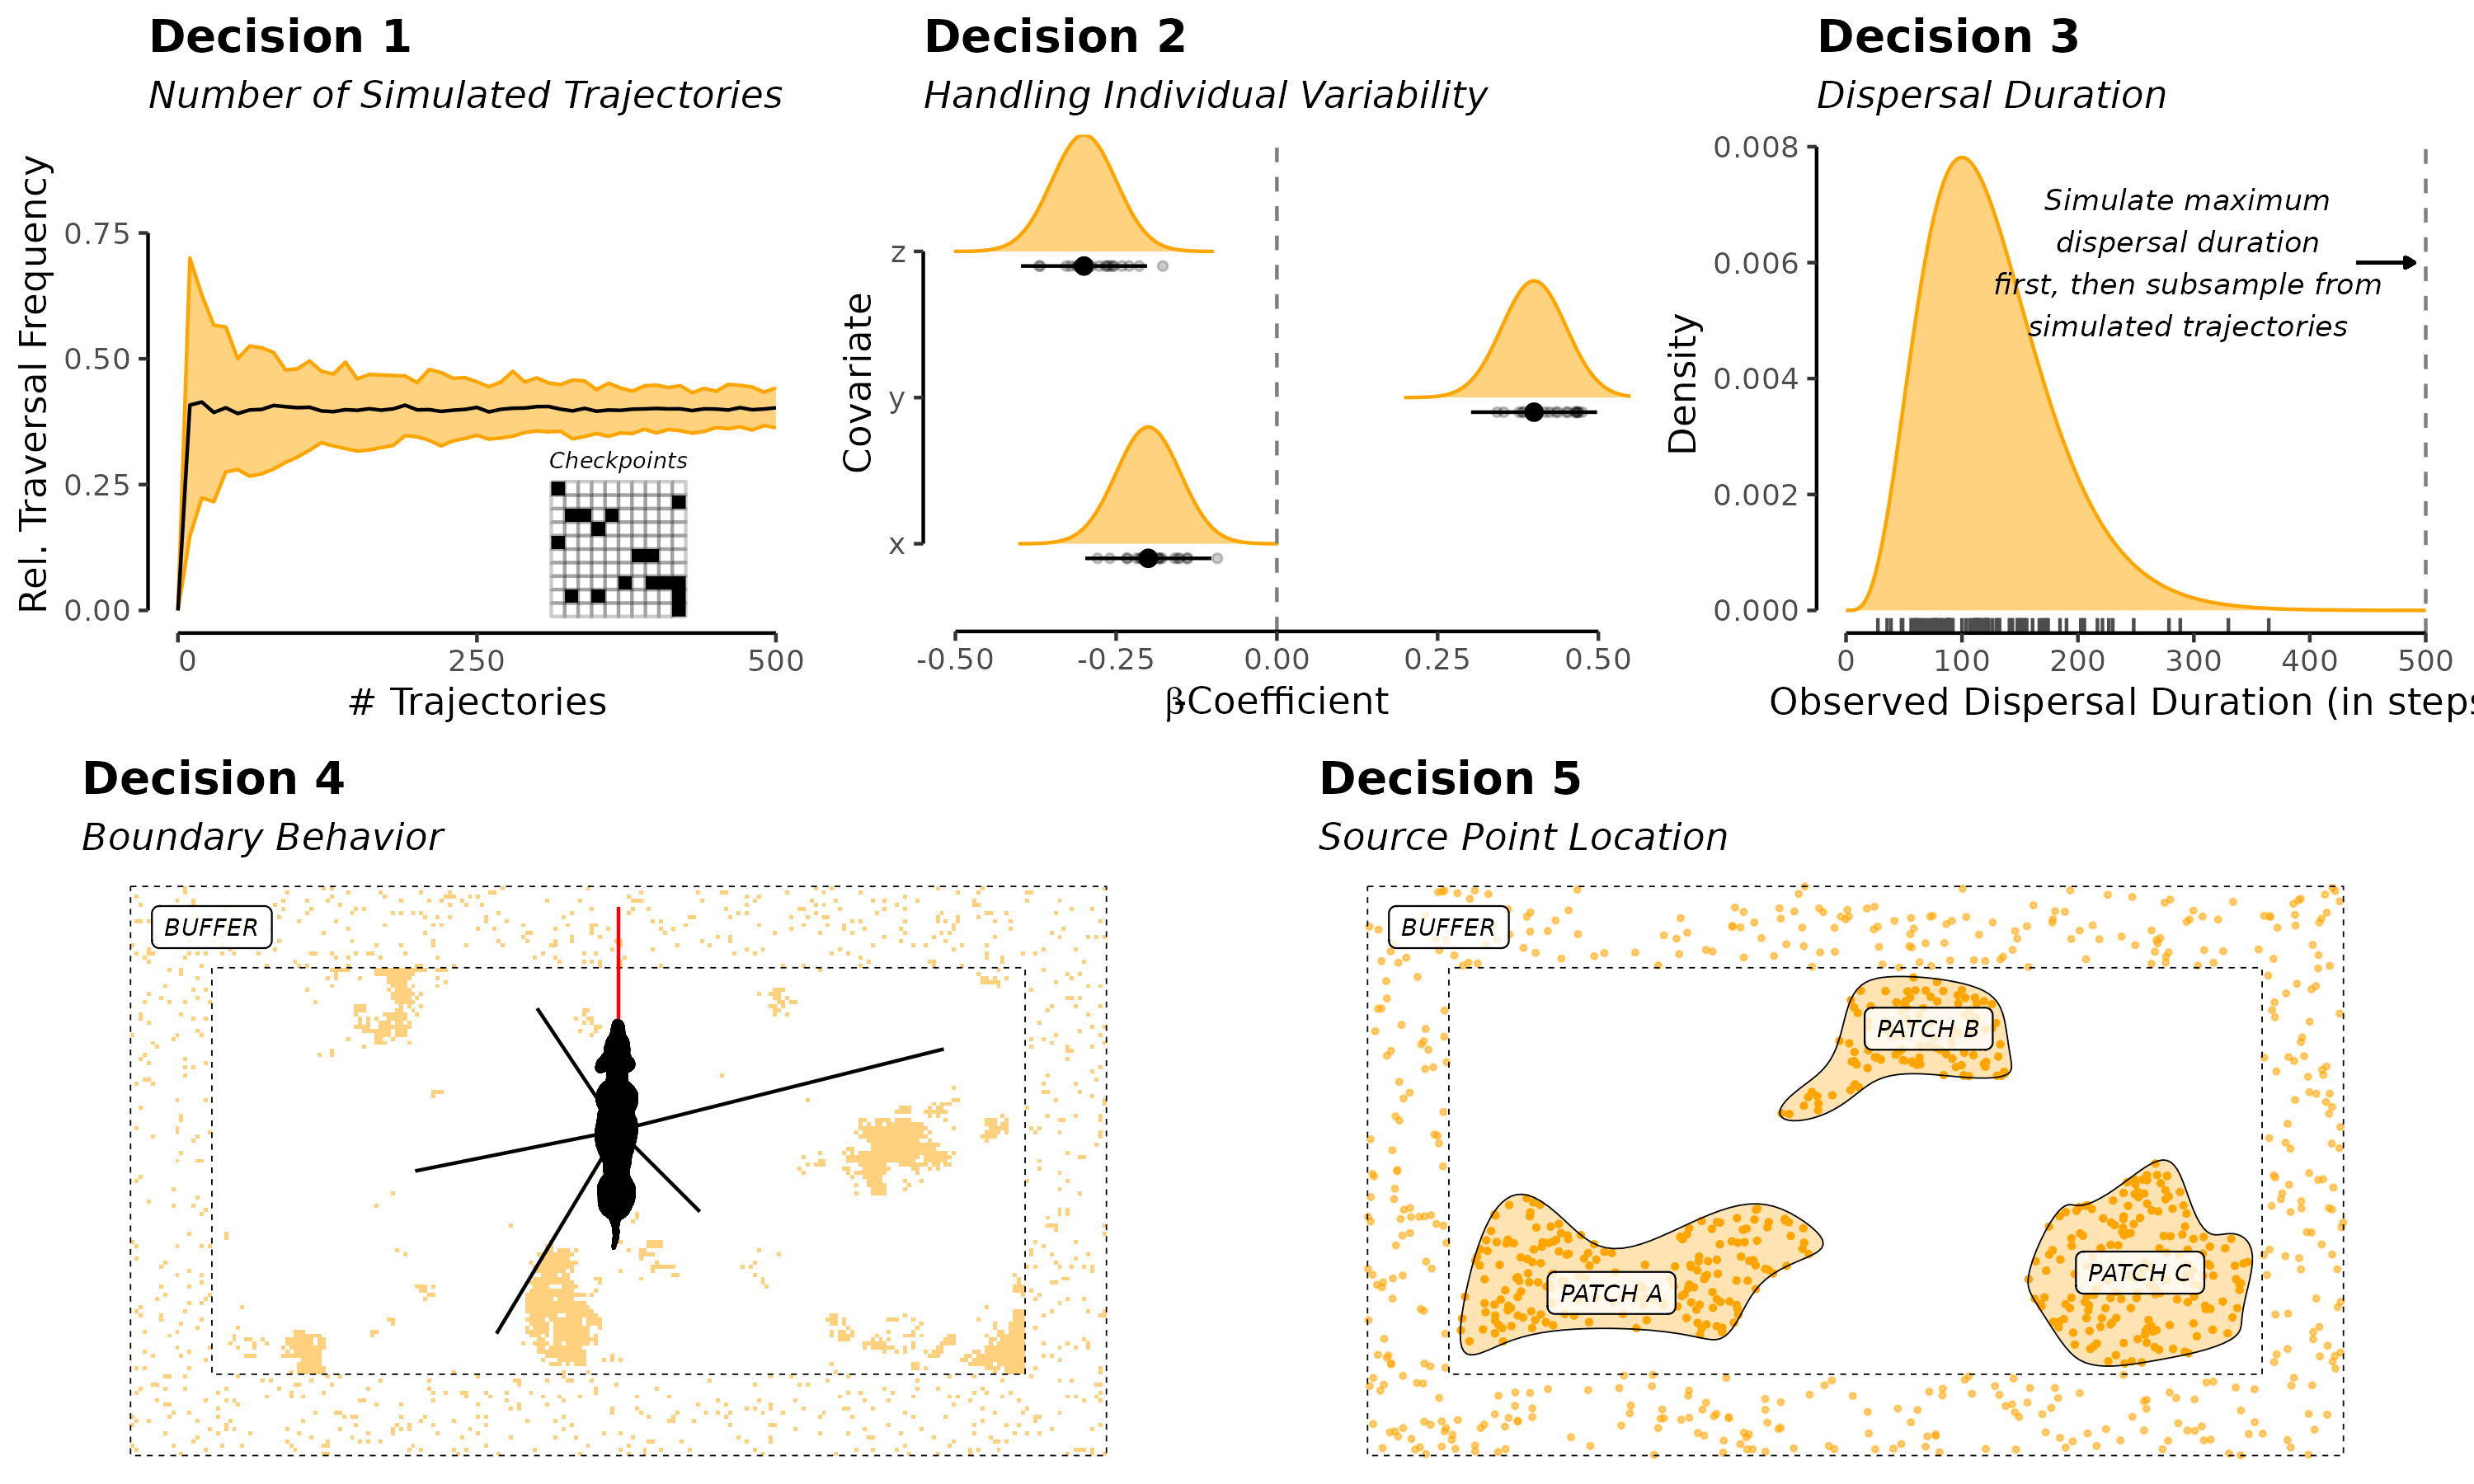
\includegraphics[width = \textwidth]{Figures/ModelingDecisions.png}
  \caption{When simulating dispersal trajectories using IBMMs, a modeler needs
  to consider several design choices. This includes the choice of the number of
  simulated trajectories (Decision 1), how to handle individual variability in
  habitat and movement preferences (Decision 2), as well as the selection of a
  dispersal duration (Decision 3). Finally, the modeler needs to define how
  individuals behave at map borders (Decision 4), and the location of source
  points from which dispersal is simulated (Decision 5).}
  \label{ModelingDecisions}
  \end{center}
\end{figure}

While many studies focus on documenting the current state of connectivity for
their study system, only few dare to pose the question: ``what could be?'' By
this, I don't simply mean how connectivity might evolve in response to
anticipated conditions under climate change, but rather how conditions could be
actively manipulated to enhance connectivity. This is insofar interesting in
that connectivity modeling is usually viewed as a means to help decision makers
improve, rather than simply preserve, connectivity \citep{Heller.2009,
Rudnick.2012}. As such, connectivity models could serve to inform the creation
of new corridors that facilitate dispersal between existing but isolated areas.
A focus on potential connectivity is particularly relevant in light of the
realization that many historically relevant movement routes have been disrupted
and vanished due to human activity. In northern Botswana, for instance, the
erection of various veterinary cordon fences in the 1960s led to a stop in
wildebeest (\textit{Conochates taurinus}) and zebra (\textit{Equus quagga})
migrations, which only resumed upon destruction of the fences in 2004
\citep{Bartlam-Brooks.2011, Bartlam-Brooks.2013}. While this case is
well-documented and the underlying causes of reduced connectivity were known,
there are many instances where the loss of crucial corridors remained unnoticed,
resulting in an overall reduction of terrestrial animal movements across the
globe \citep{Tucker.2018}. Using appropriate methods, connectivity studies could
help to reveal areas where the negative consequences of habitat fragmentation
could be reversed via restoration measures, allowing to re-establish previously
existing connectivity. Along this vein, \citet{Cushman.2010a} predict movement
corridors for African elephants in the absence of humans, thereby attempting to
reveal historically relevant dispersal routes. For the same species,
\citet{Bastille-Rousseau.2018a} employ an algorithmic approach to pinpoint areas
that appear particularly well-suited to construct wildlife crossing features to
help mitigate the detrimental impacts of roads on connectivity. Future studies
could develop similar approaches that allow randomizing or permuting current
landscapes to identify regions where enhanced connectivity could be achieved
with minimal efforts.

\section{Ecological Considerations and Limitations}

While working on the various chapters, I repeatedly had the impression that the
movement behavior of dispersing AWDs was only marginally driven by environmental
factors. This was insofar frustrating, as environmental data constituted the
only covariate data available to me at meaningful spatial scales. Although
significant selection or avoidance patterns towards certain features were
evident (e.g., water, human influence) they were generally weak. This became
particularly evident in \Cref{ChapterSeasonality}, where any benefits gained
from moving from a static to a dynamic representation of the landscape were
strongly diminished by the inclusion of additional interactions that
predominantly accounted for AWDs' circadian cycle and their tendency to move
less during hot periods. As alluded to in \Cref{ChapterSeasonality}, I suspect
that a combination of three factors explains the relatively weak association
between AWDs and their environment. Firstly, I kept my representation of land
cover rather basic. This was primarily due to the fact that I had to use
categories that were consistent across countries, which meant that I needed to
limit myself to relatively simple categories. For example, my representation of
vegetation comprised only three continuous covariates, including the percentage
cover of forest, shrubs/grassland and bare-land. In reality, the Okavango Delta
ecosystem hosts a much broader variety of vegetation patterns. Unfortunately,
these remain extremely challenging to remote sense at the required spatial
scales. Secondly, the AWD can be considered as a generalist species, currently
occurring across wide range of habitat types \citep{Woodroffe.2020}. The species
thus seems little limited by environmental factors. This particularly applies to
dispersing individuals, which only remain in a specific area for a short time,
thus exhibiting a higher tolerance towards unsuitable conditions
\citep{ONeill.2020}. This brings me to the third point; throughout the chapters,
I have exclusively utilised data collected on dispersing AWDs. As dispersers are
in search of a suitable territory and possible mates, intra- and inter-specific
factors likely play a significant role, potentially outweighing the influence of
the landscape. AWDs are weaker competitors, finding it difficult to prevail
against lions and hyenas \citep{Creel.1996, Creel.2002, Droge.2017,
Marneweck.2022}. Therefore, it can be expected that the presence of competitors
deters dispersers that are in seek of a vacant territory. Similarly, dispersers
will likely avoid areas already occupied by established packs because dispersal
coalitions are easily outnumbered by resident groups. Besides this, dispersing
coalitions are in search of potential mates, suggesting that their movement is
also driven by the availability of other-sex individuals. Considering the low
density at which the species occurs, locating mates must represent a tremendous
challenge \citep{Masenga.2016, Woodroffe.2020}. The mechanisms that facilitate
mate-finding are presently unknown, but shared marking sites are believed to
play a pivotal role \citep{Apps.2022, Claase.2022}. The notion that dispersal is
influenced not only by biophysical factors but also by ``social cues'' is
generally referred to as the ``social resistance hypothesis'', which presumes
that species are embedded into an intra- and inter-specific landscape
\citep{Armansin.2020}. Corresponding scientific evidence that supports this
hypothesis was provided by \citet{Cozzi.2018}, who concluded that social factors
may exert an even greater influence on dispersal movements than landscape
characteristics. A better understanding of the importance of such ``social
cues'' could improve our ability to more reliably predict dispersal movements,
yet necessitates appropriate data on the presence or absence of other animals.
In \Cref{CameratrapSurvey} of the Appendix, I will outline the implementation of
a cameratrap project that aims to fill this gap by collecting novel information
on large mammals across BPC's historic study area. In a future analysis, the so
collected data could be used to generate additional spatial layers that allow
modeling the influence of other species on AWD dispersal movements.

% The observed movements of an animal can be viewed as the result of the process
% in which the animal tries to minimize the distances to the things it desires.
% These things include food, shelter and potential mating partners. Dispersing
% individuals are probably particularly driven by potential mating partners and a
% vacant territory in particular. In this context, the question arises as to which
% clues dispersers use for navigation. Intra- and inter-specific factors
% presumably play a role here.

A concept closely related to the notion of ``social resistance'' is that of
``anthropogenic resistance'' \citep{Ghoddousi.2021}. It coins the idea that
anthropogenic factors can majorly alter landscape connectivity and should be
considered when studying dispersal. In \Cref{ChapterFlood}, I have encapsulated
anthropogenic resistance in two ways. First, I modeled that dispersers avoid
areas influenced by humans, thus highlighting that the mere presence of humans
can hamper connectivity. Furthermore, I overlaid predicted dispersal movements
with a human influence map, thereby disclosing potential hotspots of
human-wildlife conflict. Similar approaches were previously employed by
\citet{Cushman.2018} and \citet{Buchholtz.2020} to uncover human-wildlife
interaction hotspots for lions and African elephants, respectively. However, as
noted by \citet{Ghoddousi.2021}, an important aspect of anthropogenic resistance
is that its influence depends on human attitude. Notably, a similar degree of
human influence can result in vastly different consequences for connectivity
\citep{Ghoddousi.2021}. Using questionnaires, valuable insights into human
attitudes can be gained, enabling more informed predictions about the spatial
distribution of areas with an elevated potential for human-wildlife conflict
\citep{Feldmeier.2024}. \citet{Behr.2017}, for instance, conducted
questionnaires to develop a socio-ecological model, highlighting areas where
both environmental and anthropogenic factors favored the re-establishment of
wolves (\textit{Canis lupus}) in Switzerland. Along a similar vein,
socio-ecological connectivity models could serve to map dispersal routes
accepted by humans.

Throughout all chapters, I simulated individuals for predefined dispersal
durations, thus ignoring mortality. However, several studies have shown that
this can lead to an overestimation of dispersal success and therefore an
overestimation of connectivity \citep{Kramer-Schadt.2004, FletcherJr..2019,
Day.2020}. There are two ways in which mortality could enter my simulation
framework. First, it could be modeled as a binomial draw with constant
probability that determines whether an animal survives or dies at each simulated
step. This would merely shorten simulated dispersal paths, thus affecting
inferred connectivity patterns in relative terms. In fact, the same effect could
be achieved by simulating dispersal for a shorter duration, although this does
not capture the same level of stochasticity that would result from using a
``coin flip'' approach. Alternatively, mortality could enter the framework
spatially explicitly, reflecting the fact that mortality likely varies between
areas. \citet{Kramer-Schadt.2004}, for instance, used an IBMM where lynx
(\textit{Lynx lynx}) mortality was assumed to be higher in areas with dense road
networks. \citet{FletcherJr..2019} and \citet{Day.2020} followed a similar
approach and incorporated mortality via spatially explicit ``mortality layers'',
which consolidate various sources of mortality, such as predation, starvation
and human-wildlife conflict. However, spatially mapping the mortality risk
requires adequate data, which were lacking for my study system. Additionally,
mortality may further vary with individual (e.g., sex, age), social (e.g.,
dispersal coalition size), and environmental (e.g., temperature) factors
\citep{Behr.2023}. Ultimately, the impact of mortality on dispersing AWDs may be
buffered, given that AWDs disperse in coalitions; a single individual perishing
therefore does not imply a failure of the coalition's dispersal attempt. It is
also worth noting that mortality cannot be incorporated into traditional
connectivity models, because these do not simulate movement explicitly. The
ability to account for mortality should therefore be viewed as another major
benefit of using IBMMs over traditional models \citep{Diniz.2019}.

In this thesis, I focused on the influence of various factors on the movement
behavior of dispersing individuals, but have ignored any demographic
consequences of dispersal for metapopulation viability. Yet, such demographic
considerations are of vital importance to design more effective conservation
networks. After all, the protection of movement corridors is only meaningful if
these significantly contribute to metapopulation persistence. The movement model
parameterized in this thesis therefore serves an important component to an
individual-based population viability analysis, in which dispersal is reproduced
mechanistically and spatially realistically. Such a model could, for example, be
used to explore the demographic consequences of land protection and conversion
through hypothetical scenarios. A suitable demographic model for my study system
was parametrized by Dominik Behr as part of his PhD thesis \citep{Behr.2021}. In
order to combine the two models, we currently lack information on two processes:
settlement and home ranging behavior. A better representation of these two
processes is necessary to delineate possible home ranges and determine under
which conditions a dispersal coalition settles. Once these processes are better
understood, the combined models can be used to simulate how dispersing animals
move between subpopulations, allowing to estimate their impact on different
demographic components.

\section{Conclusion}

In conclusion, this thesis provided comprehensive exploration into the
assessment of functional landscape connectivity via individual-based dispersal
simulations, using dispersing AWDs as an example system. Through the development
and application of new methodologies, as well as by incorporating multiple
previously disregarded factors, several key insights have been gained:

\begin{itemize}

  \item \textbf{Integration of Novel Approaches:} I introduced a novel method to
  assess functional landscape connectivity via simulated dispersal from an IBMM
  parameterized via iSSFs. This approach offers a more mechanistic understanding
  of connectivity compared to traditional methods, overcoming the limiting need
  for a permeability surface and enabling the preparation of a complementary
  suite of connectivity metrics that provide a more nuanced view of functional
  connectivity.

  \item \textbf{Comprehensive Understanding of Connectivity:} By examining
  factors such as flooding conditions and seasonality, I have comparatively
  investigated how changes in landscape conditions can alter connectivity
  patterns for dispersing animals, thus highlighting the need for adopting a
  more dynamic view on landscape characteristics. Importantly, I suggested to
  not limit functional connectivity to a single dimension, but to distinguish
  between connectedness, conductance, and betweenness, thereby allowing for a
  more holistic assessment of connectivity.

  \item \textbf{Challenges and Future Directions:} Despite the many benefits
  they bring about, I have also acknowledged challenges and limitations
  associated with IBMM-based connectivity studies. This included substantial
  data requirements, computational demands, and the need for well-informed
  modeling decisions. Moving forward, I emphasized the importance of
  incorporating mortality into the simulation-process and to utilize iSSF-based
  IBMMs to gauge the demographic consequences of dispersal and connectivity. I
  also called for the inclusion of intra- and inter-specific factors  into
  connectivity models, as well as a more detailed representation of
  anthropogenic resistance that acknowledges the importance of human attitude
  towards wildlife.

\end{itemize}

Overall, this thesis contributes significantly to the fields of movement and
landscape ecology, as well as to conservation science in general, by advancing
methodologies, providing insights into the movement behavior of dispersing
individuals, and offering recommendations for future research and conservation.

\ifSubfilesClassLoaded{%
  \newpage
  \begin{singlespacing}
  \ifthenelse{\boolean{usebiblatex}}{
    \begin{refcontext}[sorting=nyt]
    \printbibliography
    \end{refcontext}
  } {
    \bibliography{../LiteratureBibtex}%
  }
\end{singlespacing}
}{}

\end{document}
